%----------------------------------------------------------------------------------------
%	PACKAGES AND THEMES
%----------------------------------------------------------------------------------------
\documentclass[aspectratio=169,xcolor=dvipsnames]{beamer}
\usetheme{Simple}

\usepackage{hyperref}
\usepackage{graphicx} % Allows including images
\usepackage{booktabs} % Allows the use of \toprule, \midrule and \bottomrule in tables
\usepackage{tikz}
\usepackage{colortbl}
\usepackage{verbatim}
\usepackage{fontawesome}
\usepackage[spanish, es-tabla]{babel}
\setbeamerfont{section in toc}{size=\fontsize{10}{12}}
\setbeamerfont{subsection in toc}{size=\fontsize{8}{12}}

\setbeamertemplate{section in toc}{\hspace*{1em}\inserttocsectionnumber.~\inserttocsection\par}
\setbeamertemplate{subsection in toc}{\hspace*{2em}\inserttocsectionnumber.\inserttocsubsectionnumber.~\inserttocsubsection\par}

\setbeamertemplate{caption}[numbered]


\renewcommand{\thefootnote}{\Roman{footnote}}



\definecolor{blue1}{cmyk}{1,0.7,0.3,0}
\definecolor{orange}{rgb}{1,0.647,0}

%----------------------------------------------------------------------------------------
%	TITLE PAGE
%----------------------------------------------------------------------------------------

% The title
\title[]{Análisis de las estimaciones de costos. \\ Agosto 2022 - Agosto 2023}
\subtitle{}

\author[] {
\includegraphics[width=0.4\textwidth]{background/ondyne_logo.png}}
\institute[NTU] 
{
    
    \textbf{\textcolor{Black}{Departamento de ingeniería}}
    \vskip 3pt
}
\date{\textcolor{Black}{Septiembre 2023}} % Date, can be changed to a custom date




\usepackage{textpos}
\addtobeamertemplate{frametitle}{}{ \begin{textblock*}{100mm}(.8\textwidth,-1cm)

\includegraphics[height=1cm,width=2.6cm]{background/ondyne_logo_blanco.png}
\end{textblock*}}



%----------------------------------------------------------------------------------------
%	PRESENTATION SLIDES
%----------------------------------------------------------------------------------------
\usebackgroundtemplate{ 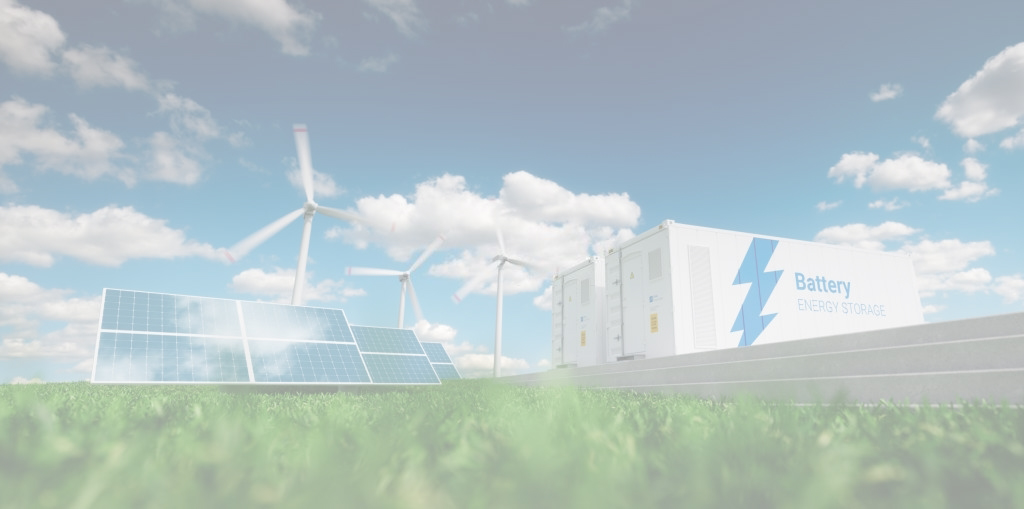
\includegraphics[width=1.1\textwidth,height= 1.1 \paperheight]{background/fondo_40.jpg}}


\begin{document}

\begin{frame}
    % Print the title page as the first slide
    \titlepage
\end{frame}
%------------------------------------------------------------------
\usebackgroundtemplate{

\includegraphics[width=\textwidth,height= 1.1 \paperheight]{background/blanco.png}}

\setbeamertemplate{footline}{%
  \leavevmode%
  \hbox{\begin{beamercolorbox}[wd=.5\paperwidth,ht=2.5ex,dp=1.125ex,leftskip=.3cm plus1fill,rightskip=.3cm]{author in head/foot}%
    \usebeamerfont{author in head/foot} Análisis de estimación de costos
  \end{beamercolorbox}%
  \begin{beamercolorbox}[wd=.5\paperwidth,ht=2.5ex,dp=1.125ex,leftskip=.3cm,rightskip=.3cm plus1fil]{title in head/foot}%
    \usebeamerfont{title in head/foot} \hfill\insertframenumber/\inserttotalframenumber
  \end{beamercolorbox}}%
  \vskip0pt%
}

\begin{frame}{Contenidos.}
    \tableofcontents
\end{frame}

%------------------------------------------------------------------
\section{Datos generales sobre la estimación de costos.}

\begin{frame}{Datos generales de las cotizaciones.}


\begin{columns}[c]
 \column{.1\textwidth}
 \column{.8\textwidth}
\begin{block}{Información general de estimaciones de costos.}
\begin{itemize}
    \item \textbf{Mes de análisis}: Agosto 2023
    \item \textbf{Período de referencia}: Agosto 2022 - Julio 2023 
    \item \textbf{Cantidad total de estimaciones$^{*}$}: 310
    \item \textbf{Monto total cotizado$^{*}$}: \$1.099.205.518
    \item \textbf{Cantidad total de clientes$^{*}$}: 148
\end{itemize}
\end{block}
\begin{block}{}
    \footnotesize{*Considera el mes de análisis y, además, el período de referencia.}
\end{block}
 \column{.1\textwidth}
\end{columns}


\end{frame}



%------------------------------------------------------------------
\section{Datos sobre las cantidades de estimaciones de costo.}
\subsection{Panorama general.}
\begin{frame}{Cantidad total cotizaciones durante el año.}


\begin{columns}[c]
 \column{.5\textwidth}
    \begin{figure}
     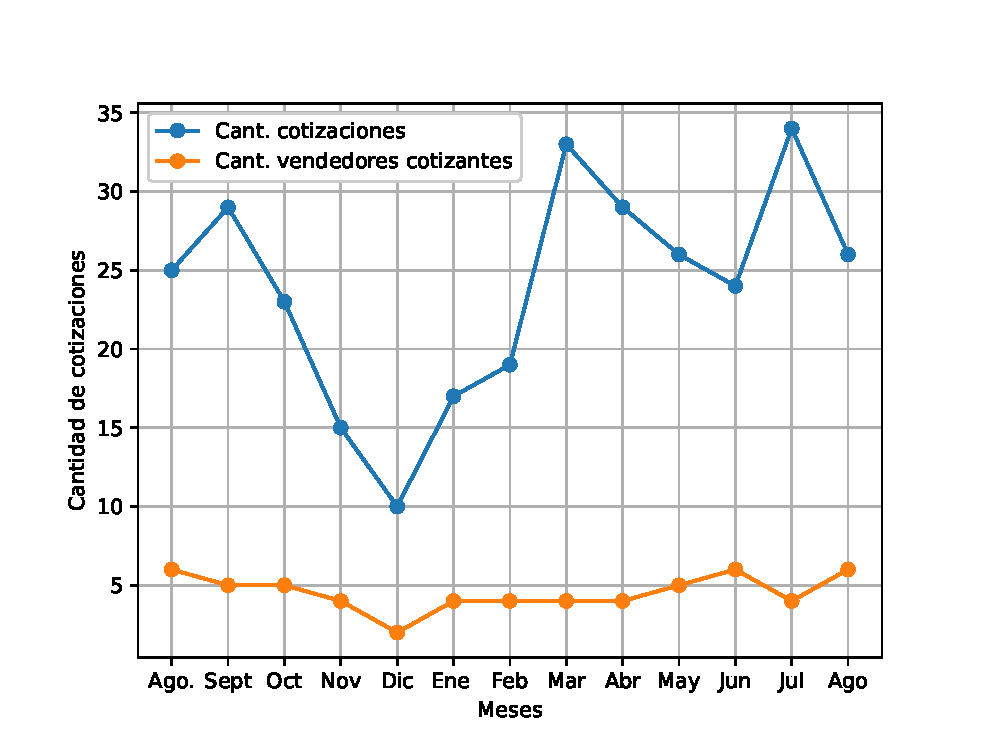
\includegraphics[width=\textwidth]{EPS/cantidad_cotizaciones_mes.eps}
     \caption{Cantidad de cotizaciones por mes.}
     \label{cotizaciones_anual}
    \end{figure}
    
 \column{.45\textwidth}
 \begin{block}{Cantidad de cotizaciones.}
 
\begin{tabular}{lcc}
                &Cant. &Por.[\%]\\
    \textbf{Cantidad este mes}: &26 &8\\
    \textbf{Total de referencia}: &284&92 \\\hline
     \textbf{Total}: &310& 100\\ 
\end{tabular}
\begin{itemize}
\footnotesize{
    \item \textbf{Promedio período ref}: 23.6
    \item \textbf{Mayor cantidad}: 34
    \item \textbf{Mes mayor cantidad}: Julio 2023
    \item \textbf{Menor cantidad}: 10
    \item \textbf{Mes menor cantidad}: Diciembre 2022}
\end{itemize}
 \tiny{*Vendedores con cotización= Total vendedores - Vendedores sin cotización.}
\end{block}

\begin{block}{}
    \scriptsize{Este mes se realizaron 2 re-cotizaciones, las que no se consideran para el análisis.}
\end{block}

\end{columns}

\end{frame}

%------------------------------------------------------------------
\subsection{Cantidad de estimaciones de costo por categoría de trabajo.}
\begin{frame}{Cantidad mensual por categoría trabajo.}

\begin{columns}[c]
 \column{.5\textwidth} 
\begin{table}[h!]
\begin{tabular}{|l|c|c|c|}\hline
  \rowcolor{MediumBlue} \color{white} Categoría & \color{white}Este mes & \color{white}Referencia* \\\hline
Integración & 8 & 4.83 \\
Mantenimiento & 5 & 5.17 \\
Servicio & 11 & 12.83 \\
Tablero & 2 & 0.83 \\ \hline
\end{tabular}
\caption{Cantidad de estimaciones de costos con respecto al promedio en el período de referencia.}
\end{table}

\begin{block}{}
    \scriptsize{*Cantidad promedio de estimaciones de costos en el período de referencia.}
\end{block}

 \column{.45\textwidth}
 \begin{figure}
     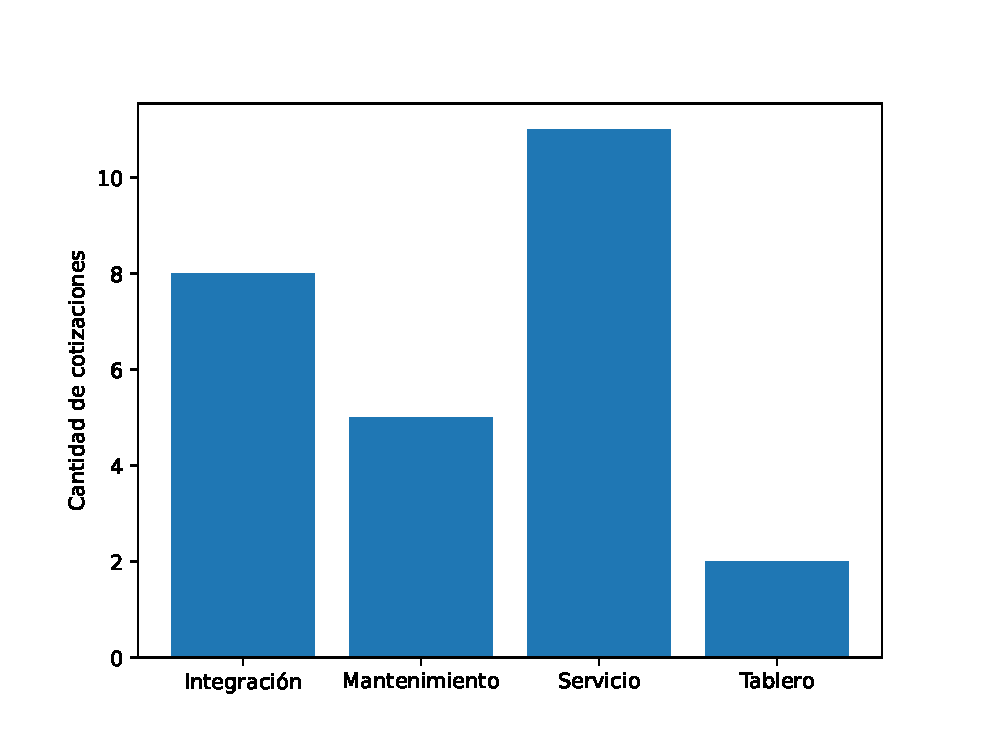
\includegraphics[width=\textwidth]{EPS/servicio_cantidad.eps}
     \caption{Distribución de la cantidad de estimaciones este mes.}
    \end{figure}

 \end{columns}
\end{frame}
%------------------------------------------------------------------
\begin{frame}{Cantidad cotizaciones por vendedor.}
\begin{columns}[c]
  \column{.45\textwidth}
 \begin{figure}
     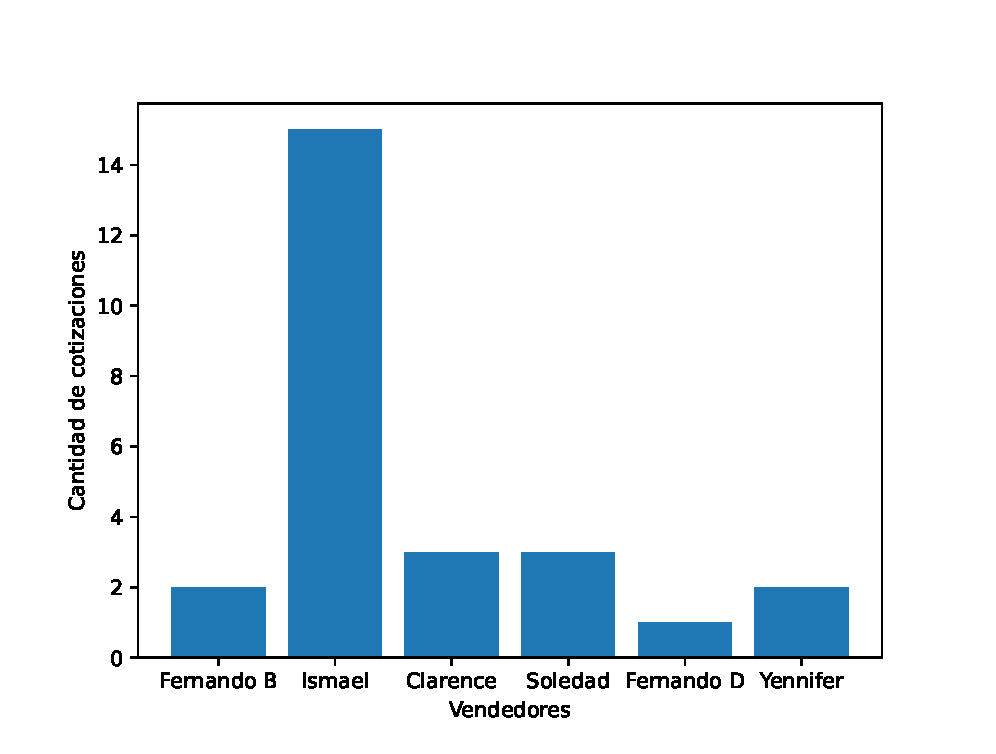
\includegraphics[width=\textwidth]{EPS/vendedor_cantidad.eps}
     \caption{Cantidad de estimaciones por cada vendedor este mes.}
     \label{graph_cantidad_estimaciones_mes}
    \end{figure}
\column{.55\textwidth} 
\begin{table}[h!]
\begin{tabular}{|l|c|c|c|c|c|}\hline
  \rowcolor{MediumBlue} \color{white}Vendedor & \color{white} Int. & \color{white} Mant.& \color{white} Serv. & \color{white} Tab. & \color{white}  Total\\\hline
Ismael & 8 & 1 & 4 & 2 & 15 \\
Fernando B & 0 & 1 & 1 & 0 & 2 \\
Clarence & 0 & 1 & 2 & 0 & 3 \\
Soledad & 0 & 1 & 2 & 0 & 3 \\
Fernando D & 0 & 0 & 1 & 0 & 1 \\
Yennifer & 0 & 1 & 1 & 0 & 2\\\hline
Total & 8 & 5 & 11 & 2 & 26\\\hline
\end{tabular}
\caption{Cantidad de estimaciones de costos este mes.}
\label{cantidad_estimaciones_mes}
\end{table}
\begin{block}{}
    \scriptsize{Este mes, el departamento de ingeniería recibió en promedio 1.4 cotizaciones por día. Considerando las re-cotizaciones.}
\end{block}
 \end{columns}

%\footnote{Considerando un mes equivalente a 20 días laborales.} 

 
\end{frame}

%------------------------------------------------------------------
\subsection{Cantidad de estimaciones de costo por departamento.}
\begin{frame}{Cantidad de cotizaciones por departamento.}
\begin{columns}[c]
 \column{.4\textwidth} 
\begin{figure}
     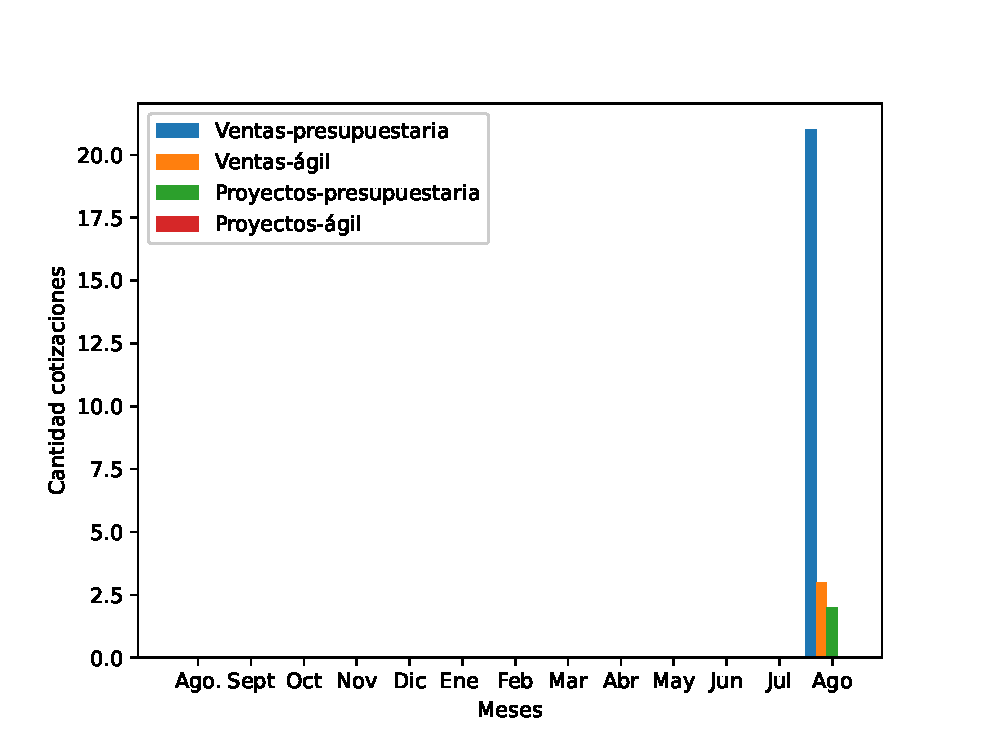
\includegraphics[width=\textwidth]{EPS/cantidad_cotizaciones_departamento_tipo.eps}
     \caption{Cantidad de cotizaciones por departamento y por tipo.}
     \label{graph:cantidad_cotizaciones_departamento_tipo}
\end{figure}

\column{.5\textwidth} 
 \begin{block}{Cantidad este mes}
     \begin{tabular}{lccc}
                    &Presupuestaria&Ágil & Total\\
          Ventas &21 & 3 &  24\\
          Proyectos&2& 0& 2\\ \hline
          Total& 23& 3 & 26\\
     \end{tabular}
\end{block}


\begin{block}{}
    \begin{itemize}
        \item El 86\% de las cotizaciones son solicitadas por el departamento de ventas.
        \item El 88\% de las estimaciones de costos son de carácter presupuestarias.
    \end{itemize}
\end{block} 

\end{columns}
\end{frame}


%------------------------------------------------------------------
\subsection{Cantidad de estimaciones de costo por rango de potencias.}
\begin{frame}{Cantidad según rango de potencias este mes.}

\begin{columns}[c]
\column{.4\textwidth} 
 \begin{block}{Resumen de este mes}
    Rango de potencia con mayor cotización en:
     \begin{itemize}
         \item \textbf{Integración}: 6-10 / 100-200 [kVA]
         \item \textbf{Mantenimientos}: 6-10 [kVA]
         \item \textbf{Servicios}: 6-10/ 100-200 [kVA]
         \item \textbf{Tableros}: 1-3/ 6-10 [kVA]
     \end{itemize}
\end{block}

\begin{block}{}
    \tiny{*El rango ``-'' se refiere a todas las cotizaciones sin potencia definida o no tiene una potencia asociada.}
\end{block} 

 \column{.55\textwidth} 
\begin{figure}
     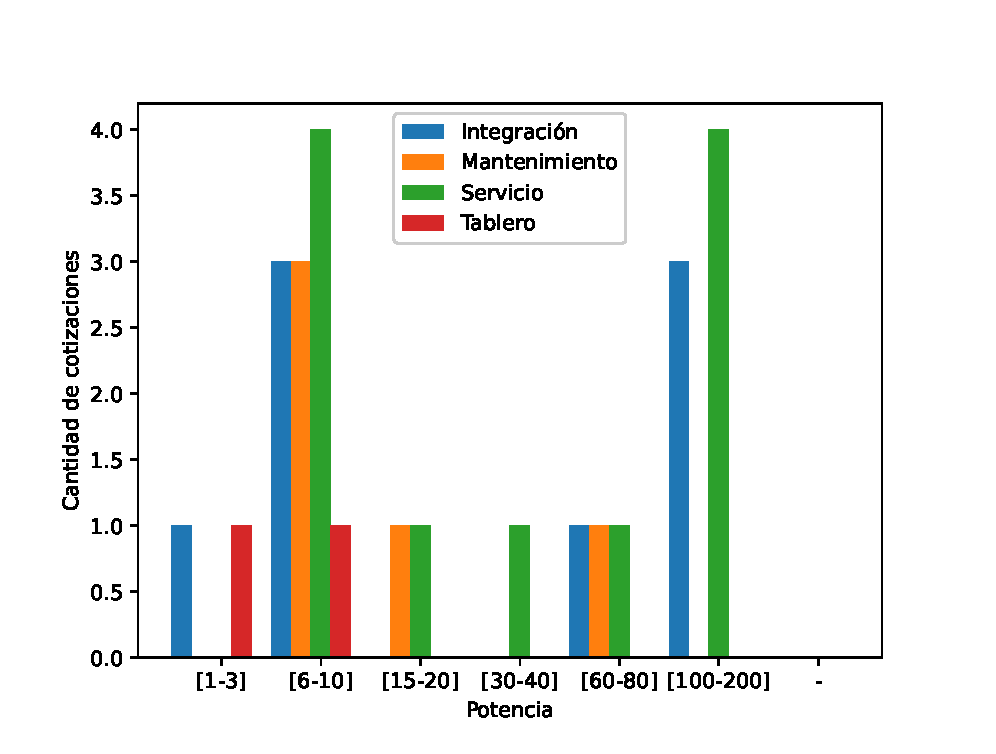
\includegraphics[width=0.9\textwidth]{EPS/potencia_mes.eps}
     \caption{Cantidad de cotizaciones según potencia este mes.}
     \label{figure:potencia_mes}
\end{figure}
\end{columns}
    
\end{frame}

%------------------------------------------------------------------

\begin{frame}{Cantidad según rango de potencias histórico.}

\begin{columns}[c]
 \column{.55\textwidth} 
\begin{figure}
     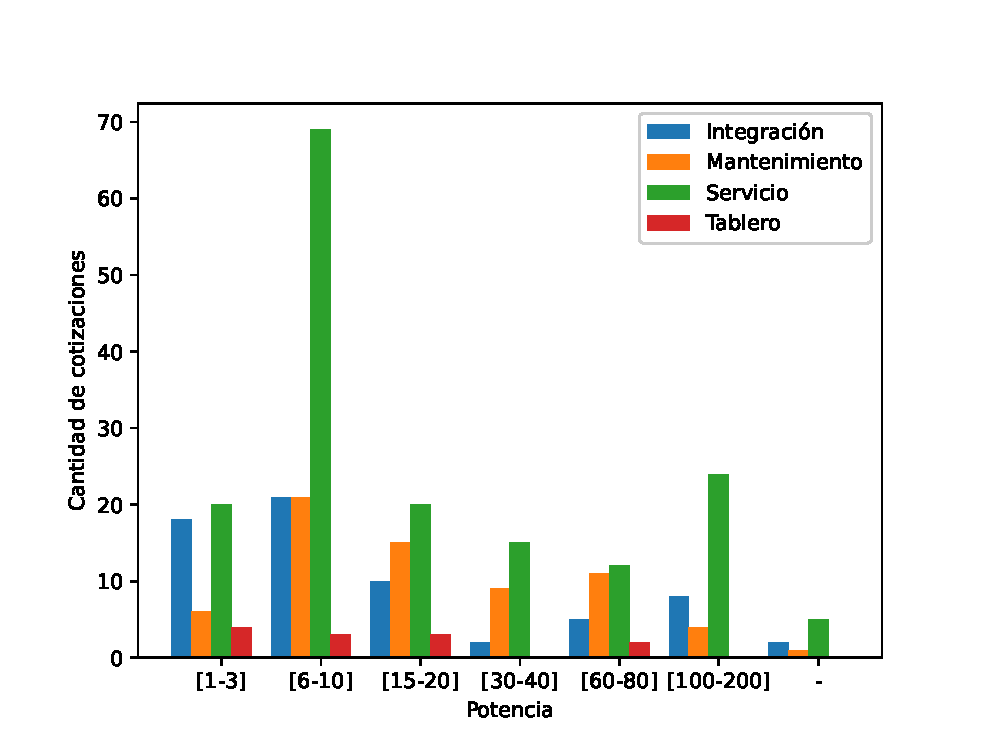
\includegraphics[width=0.9\textwidth]{EPS/potencia_historico.eps}
     \caption{Cantidad de cotizaciones según potencia histórico.}
     \label{graph:cantidad_cotizaciones_historia}
\end{figure}
\column{.4\textwidth} 
 \begin{block}{Resumen histórico$^{**}$}
    Rango de potencia con mayor cotización en:
     \begin{itemize}
         \item \textbf{Integración}: 6-10 [kVA]
         \item \textbf{Mantenimientos}: 6-10 [kVA]
         \item \textbf{Servicios}: 6-10 [kVA]
         \item \textbf{Tableros}: 1-3[kVA]
     \end{itemize}
\end{block}
\begin{block}{}
    \tiny{*El rango ``-'' se refiere a todas las cotizaciones sin potencia definida o no tiene una potencia asociada.\\
    ** Los datos históricos se refieren al mes de análisis y período de referencia.}
\end{block} 
\end{columns}
    
\end{frame}
%------------------------------------------------------------------
 \begin{frame}{Cantidad por categoría histórico.}
 \begin{columns}[c]
\column{.4\textwidth} 
 \begin{block}{Resumen histórico$^{**}$}
    Mes con mayor cotización en
     \begin{itemize}
         \item \textbf{Integración}: Julio 2023
         \item \textbf{Mantenimientos}: Julio 2023
         \item \textbf{Servicios}: Septiembre 2022
         \item \textbf{Tableros}: Septiembre 2022
     \end{itemize}
 \end{block}
 \begin{block}{}
    \tiny{** Los datos históricos se refieren al mes de análisis y período de referencia.}
\end{block}
  \column{.55\textwidth} 
 \begin{figure}
     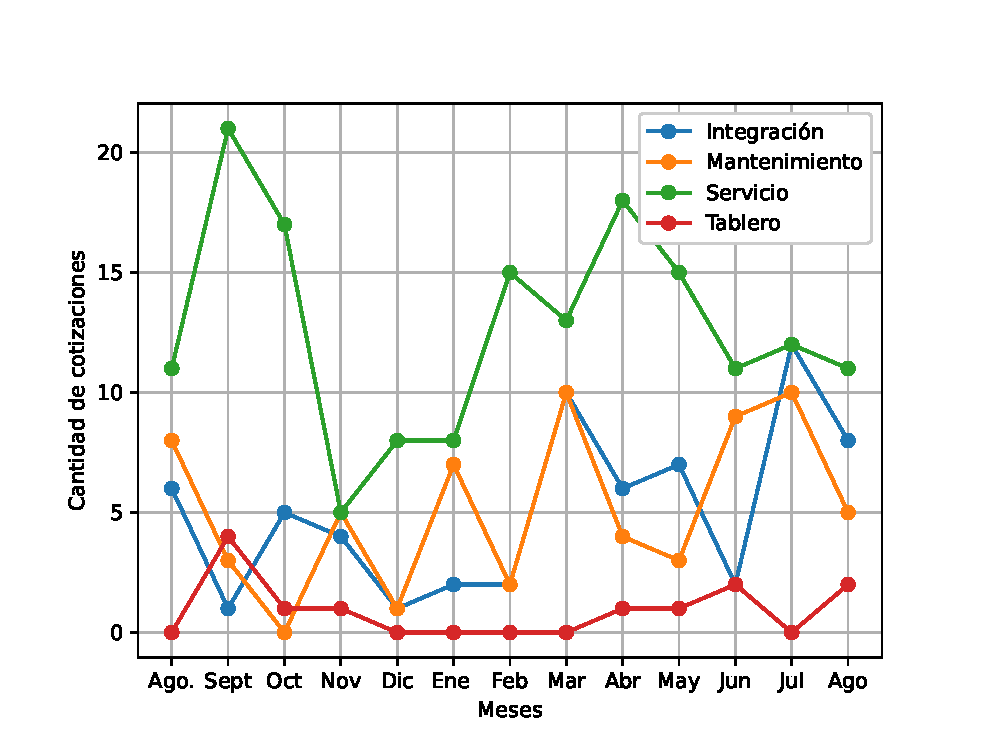
\includegraphics[width=0.9\textwidth]{EPS/servicio_cantidad2.eps}
     \caption{Resumen histórico según categoría.}
     \label{graph:resumen_hitorico_categoria}
\end{figure}
 \end{columns}
\end{frame}

%------------------------------------------------------------------
\section{Datos sobre los montos de las estimaciones de costo.}
\subsection{Panorama general.}
\begin{frame}{Costo total cotizaciones durante el año.}


\begin{columns}[c]
\column{.5\textwidth}
    \begin{figure}
     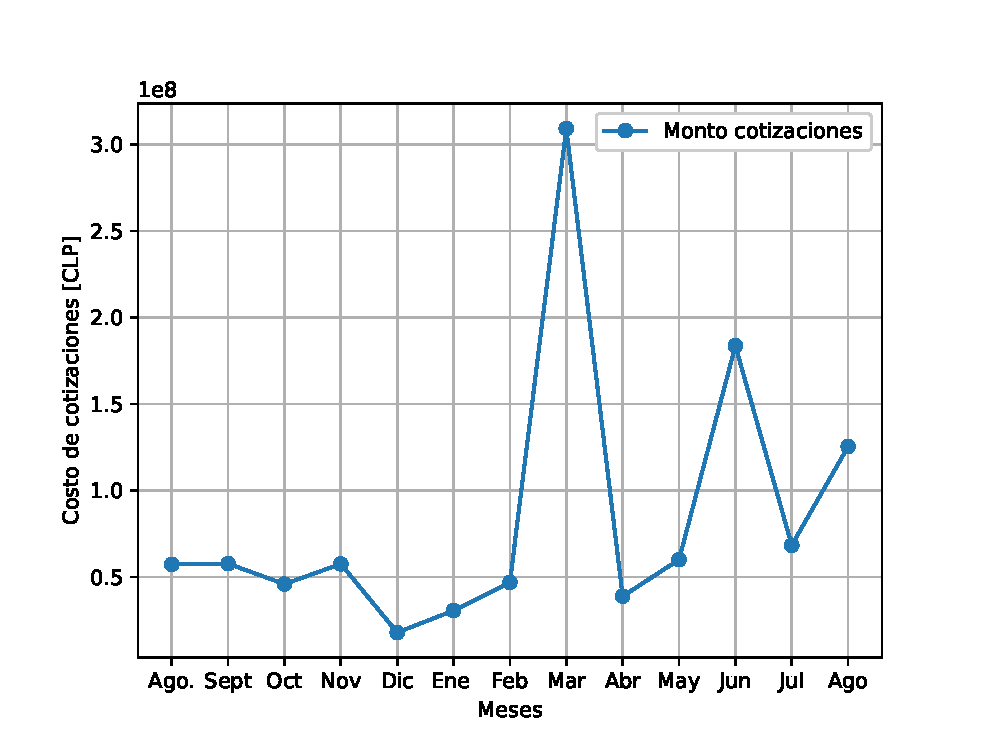
\includegraphics[width=\textwidth]{EPS/costo_cotizaciones_mes.eps}
     \caption{Costo total de cotizaciones este año.}
     \label{graph:costo_cotizaciones_mes}
    \end{figure}

 \column{.45\textwidth}
 \begin{block}{Información de costos}
 \begin{tabular}{lcc}
                & Monto & Por.[\%] \\
    \textbf{Mes}: &\$125.416.272&11\\
    \textbf{Periodo}:&\$973.789.246&89\\\hline
     \textbf{Total}: &\$1.099.205.518&100 \\ 
\end{tabular}
\scriptsize{
\begin{itemize}
    \item \textbf{Promedio período ref}: \$81.149.104
    \item \textbf{Mayor cantidad}:\$309.269.597
    \item \textbf{Mes mayor cantidad}: Marzo 2023
    \item \textbf{Menor cantidad}: \$17.883.602
    \item \textbf{Mes menor cantidad}:Diciembre 2022
\end{itemize}
}
\end{block}
\begin{block}{}
    \scriptsize{No se consideran las re-cotizaciones de este mes para el análisis.}
\end{block}
\end{columns}

\end{frame}




%------------------------------------------------------------------
\subsection{Monto de estimaciones de costo por categoría de trabajo.}
\begin{frame}{Monto de cotizaciones por categoría.}
\begin{columns}[c] 
\column{.6\textwidth} 
\begin{table}[h!]
\begin{tabular}{|l|c|c|}\hline
  \rowcolor{MediumBlue} \color{white} & \color{white}Este mes & \color{white}Referencia*  \\\hline
Integración & \$86.789.384 & \$26.341.741 \\
Mantenimiento &\$22.213.368 & \$6.741.536 \\
Servicio &  \$14.651.616 & \$45.617.673 \\
Tablero & \$1.761.904 & \$2.448.154\\\hline
\end{tabular}
\caption{Costo de estimaciones con respecto al promedio en el período de referencia.}
\label{table:costo_promedio_mensual}
\end{table}
\begin{block}{}
    \footnotesize{*Cantidad promedio de estimaciones de costos en el período de referencia.}
\end{block}

 \column{.4\textwidth} 
 \begin{figure}
     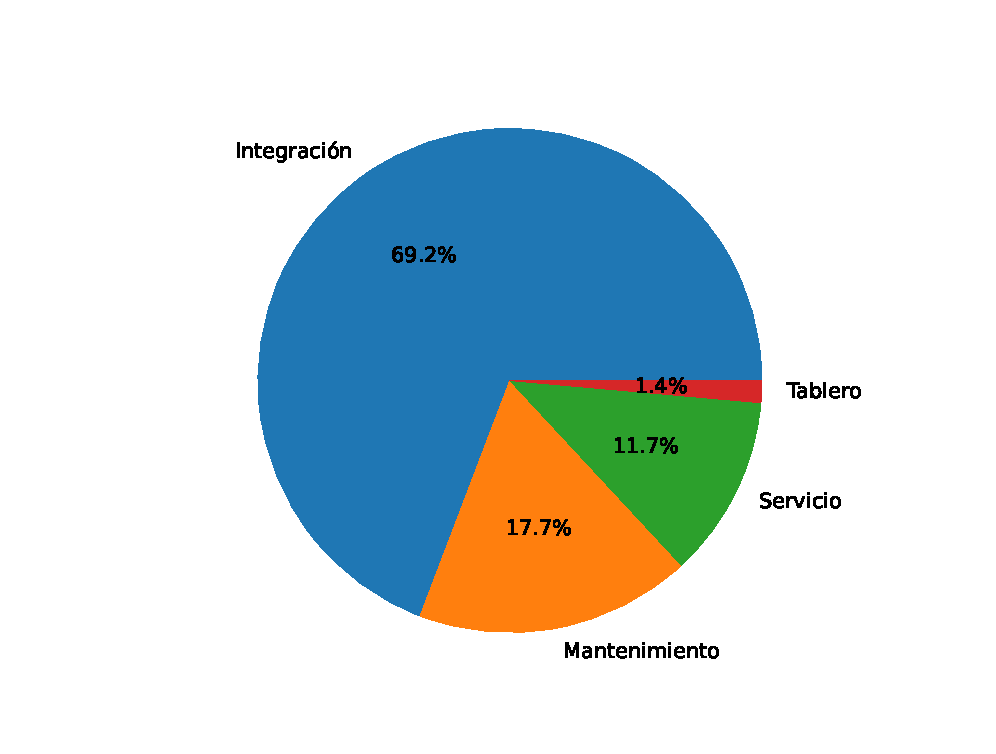
\includegraphics[width=\textwidth]{EPS/servicio.eps}
     \caption{Distribución de los costos en los distintas categorías en este mes.}
    \end{figure}

 \end{columns}
\end{frame}
%------------------------------------------------------------------

\begin{frame}{Monto cotizado por vendedor este mes.}

\begin{table}[h!]
\begin{tabular}{|l|r|r|r|r|r|}\hline
  \rowcolor{MediumBlue} \color{white}Solicitante & \color{white} Integración & \color{white} Mantenimiento& \color{white} Servicio & \color{white} Tablero & \color{white}  Total\\\hline
Ismael & \$86.789.384 & \$129.368 & \$2.200.708 & \$1.761.904 & \$90.881.364 \\
Yennifer & \$0 & \$18.593.402 & \$1.507.686 & \$0 & \$20.101.088 \\
Clarence & \$0 & \$670.344 & \$5.263.782 & \$0 & \$5.934.126 \\
Soledad & \$0 & \$441.873 & \$5.421.251 & \$0 & \$5.863.124 \\
Fernando B & \$0 & \$2.378.381 & \$18.798 & \$0 & \$2.397.179 \\
Fernando D & \$0 & \$0 & \$239.391 & \$0 & \$239.391 \\ \hline
Total & \$92.763.858 & \$22.213.368 & \$14.651.616 & \$1.761.904 & \$125.416.272
 \\ \hline
\end{tabular}
\caption{Monto cotizado por vendedor en cada categoría este mes.}
\label{table:monto_cotizado_vendedor}
\end{table}
\end{frame}

%------------------------------------------------------------------

\begin{frame}{Monto cotizado por vendedor los últimos 4 meses.}

\begin{table}[h!]
\begin{tabular}{|l|r|r|r|r|}\hline
  \rowcolor{MediumBlue} \color{white}Solicitante &\color{white} Mayo &\color{white} Junio &\color{white} Julio &\color{white} Agosto\\ \hline
Yennifer &\$ 10.828.766 &\$ 13.482.077&\$ 0 &\$ 20.101.088\\
Clarence &\$ 0 &\$ 67.667.069 &\$17.507.905 &\$ 5.934.126\\
Ismael  &\$ 40.562.906 &\$ 7.090.768&\$49.325.180&\$ 90.881.364\\
Soledad  &\$ 2.268.009 &\$ 92.169.380 &\$0 &\$ 5.863.124\\
Fernando B  &\$ 2.670.093 &\$ 2.709.157&\$1.269.379&\$ 2.397.179 \\
Fernando D  &\$ 3.645.348 &\$ 560.108 &\$229.551 &\$239.391\\ \hline
Total&\$59.975.122&\$183.678.559& \$68.332.015&\$125.416.272 \\\hline
\end{tabular}
\caption{Costo de cotizaciones por cada solicitante los últimos 4 meses.}
\label{table:cotizaciones_ultimos_4_meses}
\end{table}
\end{frame}


%------------------------------------------------------------------
\subsection{Monto de estimaciones de costo por departamento.}
\begin{frame}{Monto cotizado por departamento.}
\begin{columns}[c]
 \column{.4\textwidth} 
\begin{figure}
     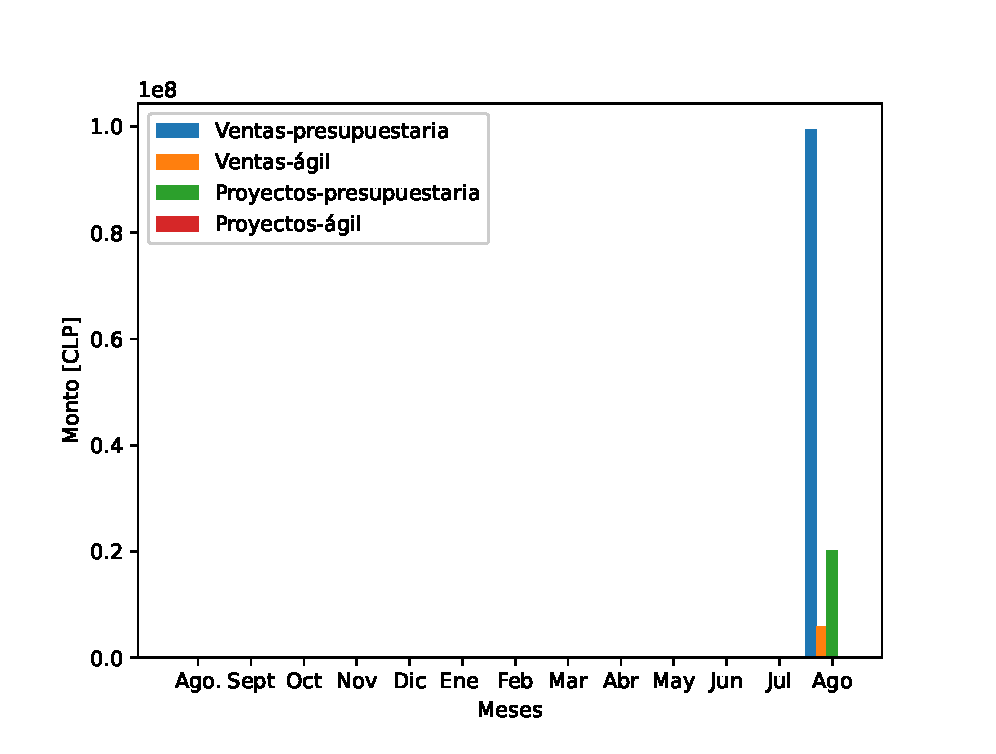
\includegraphics[width=1\textwidth]{EPS/monto_cotizaciones_departamento_tipo.eps}
     \caption{Monto cotizado por departamento.}
     \label{graph:cantidad_cotizaciones_departamento_tipo}
\end{figure}
\column{.6\textwidth} 
 \begin{block}{Costos por departamento}
     \begin{tabular}{lccc}
                    &Presupuestaria&Ágil & Total\\
          Ventas &\$99.381.058 &\$5.934.126 & \$105.315.184\\
          Proyectos&\$20.101.088&0 &\$20.101.088\\ \hline
          Total& \$119.482.146& \$5.934.126  & \$125.416.272\\
     \end{tabular}
\end{block}
\begin{block}{}
   \begin{itemize}
       \item El 84\% de los costos de las estimaciones de este mes provienen del departamento de ventas.
       \item El 95\% de los costos de las estimaciones de este mes son de carácter presupuestario. 
   \end{itemize}
\end{block} 

\end{columns}
\end{frame}



%------------------------------------------------------------------
\subsection{Monto de estimaciones de costo por rango de potencias.}
\begin{frame}{Monto por rango de potencias este mes.}

\begin{columns}[c]
\column{.35\textwidth} 
 \begin{block}{Resumen de este mes}
    Categoría con mayor costo en:
     \begin{itemize}
         \item \textbf{Integración}: 60-80 [kVA]
         \item \textbf{Mantenimientos}: 6-10 [kVA]
         \item \textbf{Servicios}: 100-200 [kVA]
         \item \textbf{Tableros}: 6-10 [kVA]
     \end{itemize}
\end{block}
\begin{block}{}
    \tiny{*El rango ``-'' se refiere a todas las cotizaciones sin potencia definida o no tiene una potencia asociada.}
\end{block} 

 \column{.6\textwidth} 
\begin{figure}
     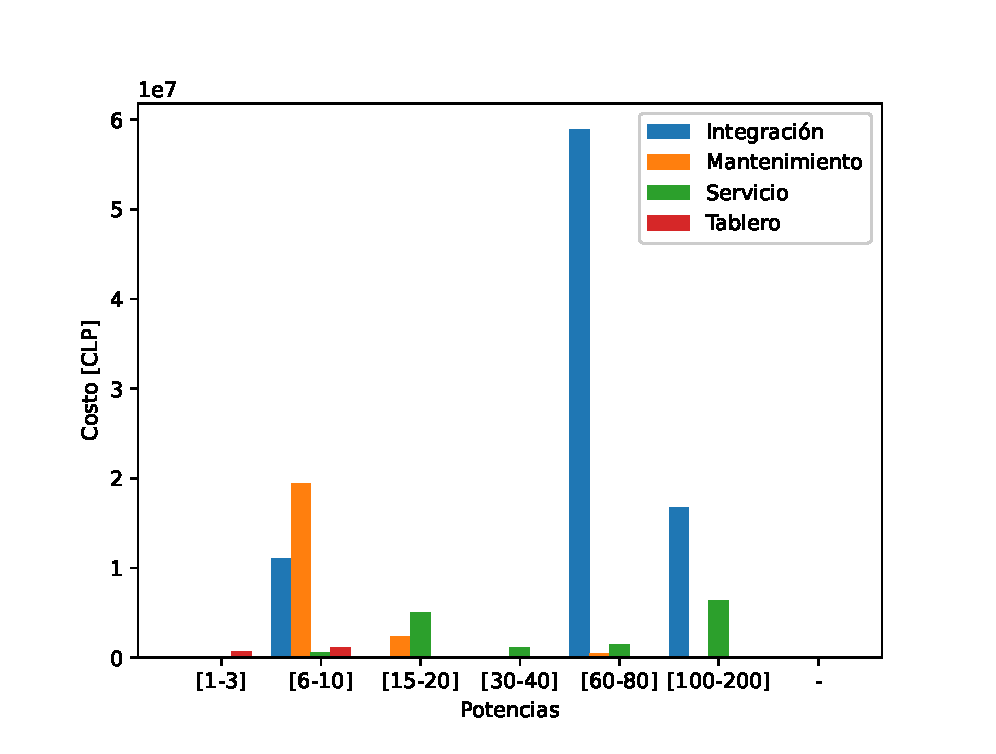
\includegraphics[width=0.85\textwidth]{EPS/potencia_costo_mes.eps}
     \caption{Monto de cotizaciones según potencia este mes.}
     \label{graph:potencia_costo_mes}
\end{figure}
\end{columns}
    
\end{frame}

%------------------------------------------------------------------

\begin{frame}{Monto por rango de categorías histórico.}

\begin{columns}[c]
 \column{.6\textwidth} 
\begin{figure}
     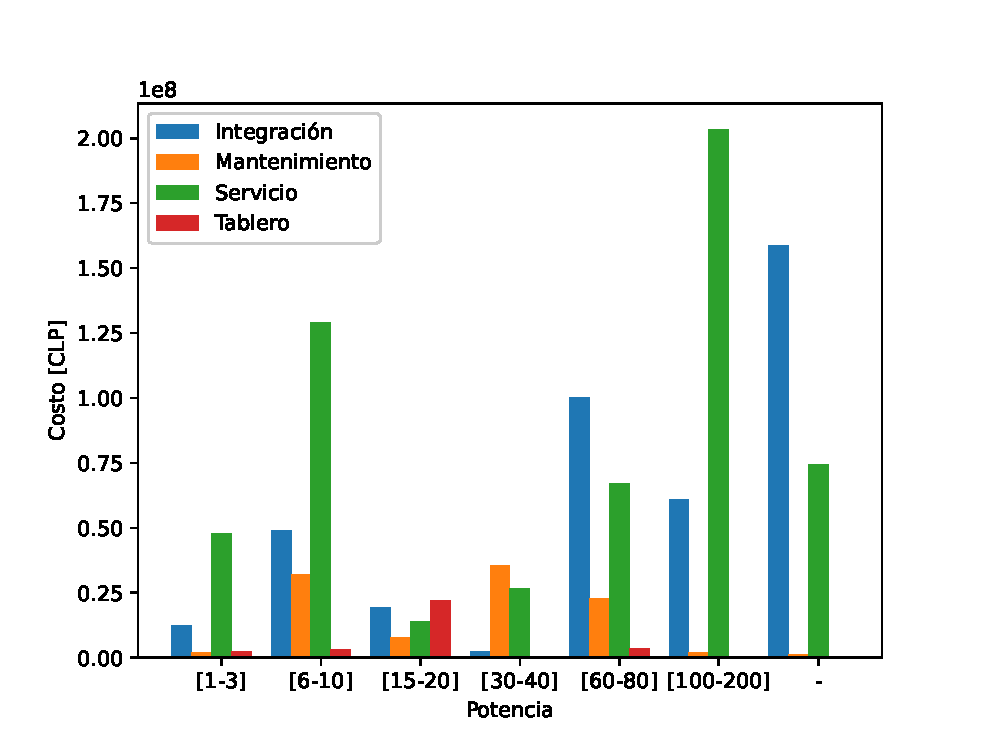
\includegraphics[width=0.85\textwidth]{EPS/potencia_costo_historico.eps}
     \caption{Monto de cotizaciones según potencia histórico}
     \label{graph:potencia_costo_historico}
\end{figure}
\column{.35\textwidth} 
 \begin{block}{Resumen histórico$^{**}$}
    Categoría con mayor costo en:
     \begin{itemize}
         \item \textbf{Integración}: - [kVA]
         \item \textbf{Mantenimientos}: 30-40 [kVA]
         \item \textbf{Servicios}: 100-200 [kVA]
         \item \textbf{Tableros}: 15-20 [kVA]
     \end{itemize}
\end{block}
\begin{block}{}
    \tiny{*El rango ``-'' se refiere a todas las cotizaciones sin potencia definida o no tiene una potencia asociada.\\
    ** Los datos históricos se refieren al mes de análisis y período de referencia.}
\end{block} 
\end{columns}
    
\end{frame}

%------------------------------------------------------------------
 \begin{frame}{Monto por categoría de trabajo.}
 \begin{columns}[c]
\column{.35\textwidth} 
 \begin{block}{Resumen histórico$^{**}$}
    Mes con mayor monto en:
     \begin{itemize}
         \item \textbf{Integración}: Marzo 2023
         \item \textbf{Mantenimientos}: Agosto 2023
         \item \textbf{Servicios}: Junio 2023
         \item \textbf{Tableros}: Abril 2023
     \end{itemize}
 \end{block}
 \begin{block}{}
    \tiny{** Los datos históricos se refieren al mes de análisis y período de referencia.}
\end{block} 
  \column{.6\textwidth} 
 \begin{figure}
     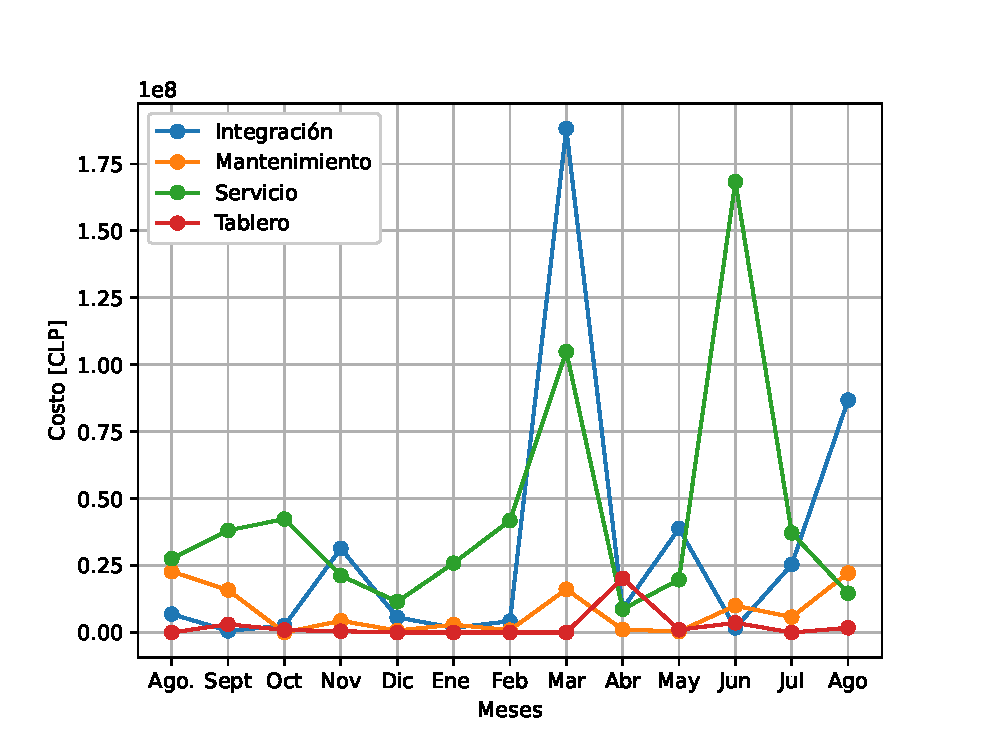
\includegraphics[width=0.85\textwidth]{EPS/servicio_monto2.eps}
     \caption{Resumen histórico según categoría.}
     \label{graph:servicio_monto2}
\end{figure}
 \end{columns}
\end{frame}


%------------------------------------------------------------------
\section{Pronósticos.}
\subsection{Proyección anterior vs valores obtenidos este mes.}
 \begin{frame}{Proyección anterior vs valores actuales.}

Valores proyectados en Julio para el mes de Agosto  
\begin{table}[h!]
    \centering
         \begin{tabular}{|l||c|c|c||c|c|c|}  \hline
          \rowcolor{MediumBlue} \color{white}Tipo &\color{white}P40&\color{white}P60& \color{white}Cant mes  &\color{white}P40&\color{white}P60&\color{white}Total mes \\ \hline
          Int& 3 & 6 &8 &\$5.371.601&\$11.479.013&\$86.789.384 \\
          Mant&4&7&5 & \$2.553.668&\$6.605.690&\$22.213.368\\
          Serv&11&13&11 &\$24.969.542&\$37.385.656&\$14.651.616\\
          Tabl &0&1&2 &\$0&971.115&\$1.761.904\\ \hline
          Total &18&27& \cellcolor{Green}26 &\$32.894.811 &\$56.441.474 & \cellcolor{Red}\$125.416.272 \\ \hline           
     \end{tabular}
    \caption{Valores esperados para el próximo mes en las diferentes categorías.}
    \label{valores_esperados}
\end{table}
 
 \begin{columns}[c]
 \column{.7\textwidth}
 

\begin{block}{}
   \scriptsize{La estimación de costos para el mes de agosto resultó inexacta debido a que algunas cotizaciones superaron significativamente el rango previsto, llegando a ser el total dos veces mayor al valor máximo esperado. Por otro lado, la cantidad total de este mes se acercó más al rango proyectado, sin embargo, solo se consiguió acertar en las categorías mantenimiento y servicio.} 
\end{block}
 \column{.2\textwidth} 
 \begin{block}{}
   \scriptsize{P40: Percentil 40 (40\%)\\
   P60: Percentil 60 (60\%)}
 \end{block}
 \end{columns}
\end{frame}


%------------------------------------------------------------------
\subsection{Proyección para el próximo mes.}

 \begin{frame}{Distribución estadística de las cantidades.}
 \begin{columns}[c]
  \column{.5\textwidth} 
 \begin{figure}
     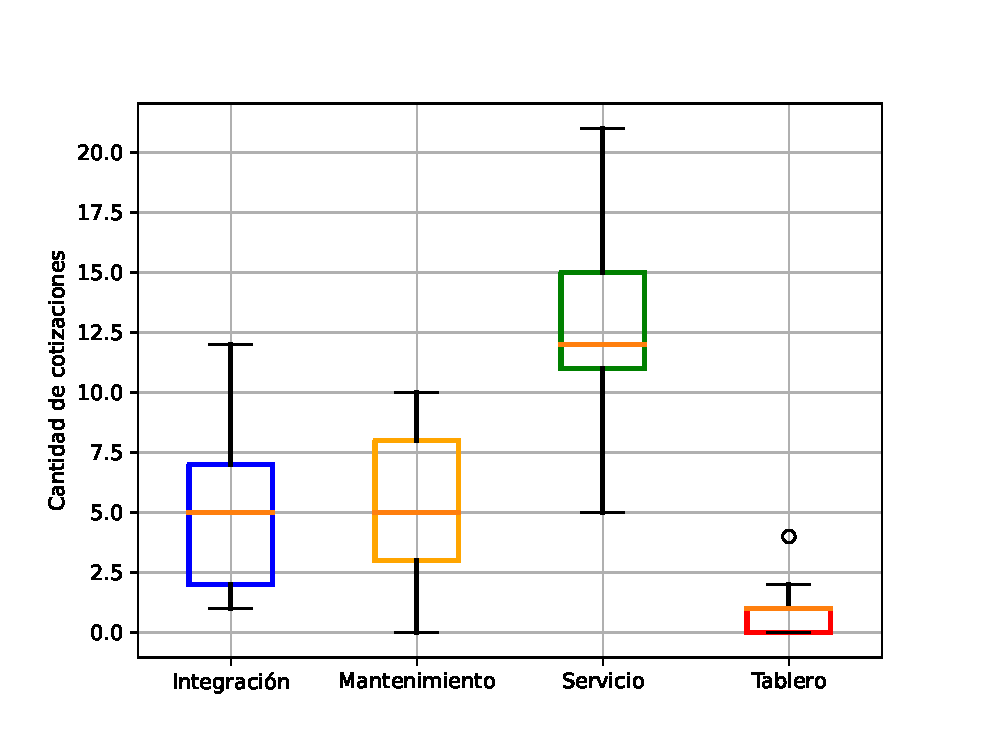
\includegraphics[width=\textwidth]{EPS/boxplot.eps}
     \caption{Distribución de la cantidad de cotizaciones según categoría.}
     \label{box_plot1}
\end{figure}
 \column{.45\textwidth} 
\begin{block}{Cantidad de cotizaciones}
     \begin{tabular}{lccc}
                    &Q1&Q2&Q3\\
          Integración:&2 & 5& 7 \\
          Mantenimiento:&3& 5&8\\
          Servicio:& 11&12 &15\\
          Tablero :& 0& 1&1\\ \hline
          Total & 16 & 23&31\\
     \end{tabular}
\end{block}
 \begin{block}{}
    \scriptsize{$^{o}$ Datos atípicos en las distintas categorías.\\
    Q1= Primer cuartil (25\%).\\
    Q2= Segundo cuartil (50\%).\\
    Q3= Tercer cuartil (75\%).}
    
\end{block}
 \end{columns}
\end{frame}


%------------------------------------------------------------------

 \begin{frame}{Distribución estadística de los montos.}
 \begin{columns}[c]
 \column{.15\textwidth}
 \column{.7\textwidth} 
\begin{block}{Costo de cotizaciones}
     \begin{tabular}{lccc}
                       & Q1 & Q2 & Q3\\ 
          Integración:&\$2.566.834 &\$6.877.728&\$31.415.399\\ 
          Mantenimiento:&\$860.161&\$4.372.809&\$15.858.660\\
          Servicio:&\$19.697.451&\$27.615.931&\$41.799.107\\ 
          Tablero :&\$0&\$491.846&\$1.761.904\\ \hline 
          Total&\$23.124.446&\$39.358.314 & \$90.835.070 \\
     \end{tabular}
\end{block}
 \begin{block}{}
    \scriptsize{Q1= Primer cuartil (25\%).\\
    Q2= Segundo cuartil (50\%).\\
    Q3= Tercer cuartil (75\%).}
\end{block}
  \column{.15\textwidth} 
 %\begin{figure}
  %   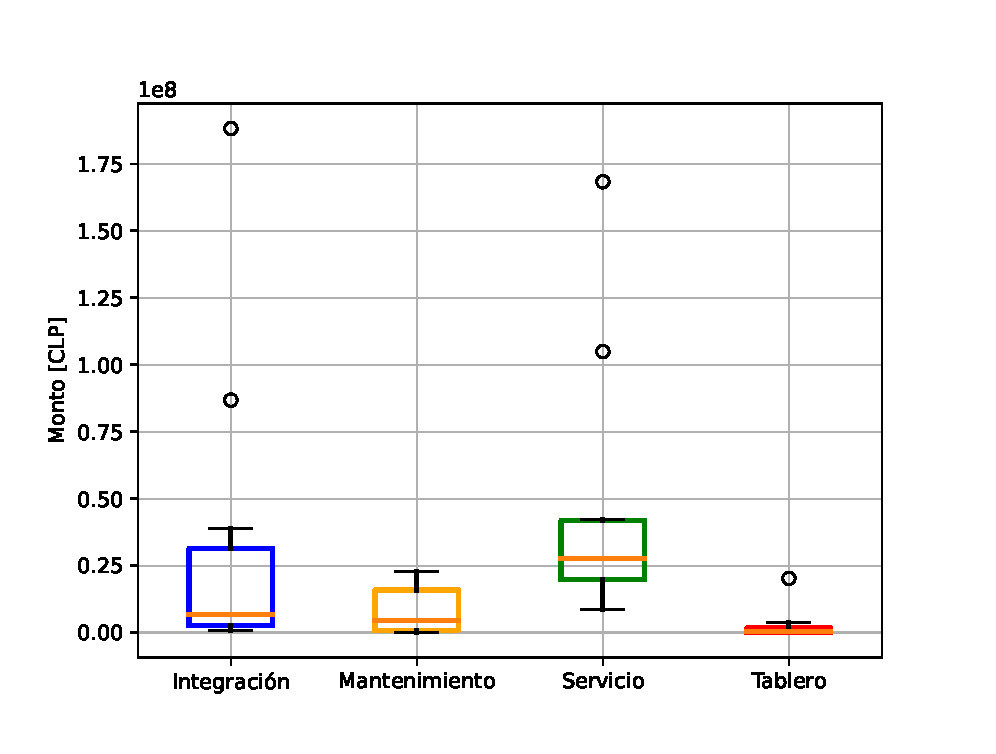
\includegraphics[width=0.85\textwidth]{EPS/boxplot2.eps}
  %   \caption{Distribución de los costos de cotizaciones según categoría}
  %   \label{boxplot2}
%\end{figure}
 \end{columns}
\end{frame}

%------------------------------------------------------------------

 \begin{frame}{Proyección para el siguiente mes.}
 \begin{columns}[c]
 \column{.15\textwidth}
  \column{.7\textwidth}
  \begin{block}{Rango de proyección para el mes de Septiembre}
     
         \begin{tabular}{l|cc|cc}
                       & P40 & P60 & P40 & P60\\ 
          Integración:&3&6&\$5.371.601 &\$12.169.551\\ 
          Mantenimiento:&4 &5 &\$2.553.668&\$6.605.690\\
          Servicio:&11 &13 &\$24.969.542&\$37.385.656\\ 
          Tablero:& 0& 1&\$0&\$971.115\\ \hline 
          Total&18 &25 &\$32.894.811&\$57.137.012\\
     \end{tabular}
       
  \end{block}

\begin{block}{}
        \scriptsize{P40= Percentil 40 (40\%).\\
    P60= Percentil 60 (60\%).}
\end{block}

 \column{.15\textwidth}
  \end{columns}
\end{frame}

%------------------------------------------------------------------
\section{Datos sobre los clientes.}
\begin{frame}{Datos sobre los clientes.}


\begin{columns}[c]
 \column{.5\textwidth}
\begin{block}{Información general}
\begin{itemize}
    \item \textbf{Clientes cotizados este mes}: 20
    \item \textbf{Clientes promedio en período ref}: 17.33
    \item \textbf{Máx clientes cotizados mensual}: 26
    \item \textbf{Min clientes cotizados mensual}: 7
\end{itemize}
\end{block}
 
\begin{block}{Cantidad clientes}
\begin{tabular}{lc}
    \textbf{Clientes nuevos de este mes}:& 11 \\
     \textbf{Clientes en el período de ref}: & 137 \\ \hline
     \textbf{Cantidad total}: & 148
\end{tabular}
\end{block}

 \column{.4\textwidth}
 \begin{block}{Clientes nuevos este mes}
     \begin{itemize}
    \tiny{
    \item Comercial Simelco
    \item Cesfam Teresa Baldecchi
    \item FACH
    \item Santander Import
    \item BC Comunicaciones
    \item Supermercado Santa Teresa Maria Pinto
    \item Consejo nacional de Televisión
    \item Metro S.A.
    \item Observatorio La Silla
    \item Edapi
    \item Cámara del comercio}
    \end{itemize}
 \end{block}
\end{columns}

\end{frame}

%\footnote{Clientes que no han cotizado durante el período de estudio}

%------------------------------------------------------------------

\begin{frame}{Cantidad de cotizaciones por cliente.}

\begin{columns}[c]
 \column{.35\textwidth}

\begin{block}{Cantidad cotizaciones histórico$^{**}$}
\begin{itemize}
    \item  HYO : 20
    \item  Itaú : 17
    \item  ISTC : 9
    \item  Aqueveque : 9
\end{itemize}
\end{block}
\begin{block}{}
    \tiny{** Los datos históricos se refieren al mes de análisis y período de referencia.}
\end{block}

 \column{.60\textwidth} 
\begin{figure}
     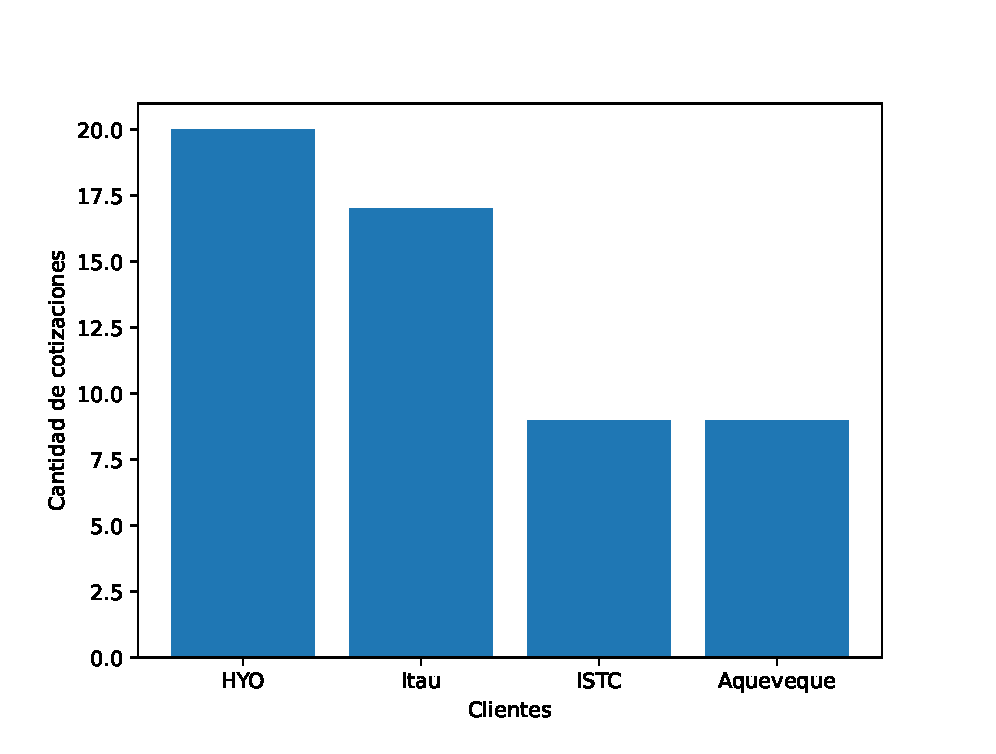
\includegraphics[width=0.8\textwidth]{EPS/cliente_cantidad_total.eps}
     \caption{Cantidad total de cotizaciones por cliente.}
     \label{graph:cotizacion_max_cliente}
\end{figure}
\end{columns}
    
\end{frame}

%------------------------------------------------------------------

\begin{frame}{Monto de cotizaciones por cliente.}

\begin{columns}[c]
  \column{.60\textwidth} 
\begin{figure}
     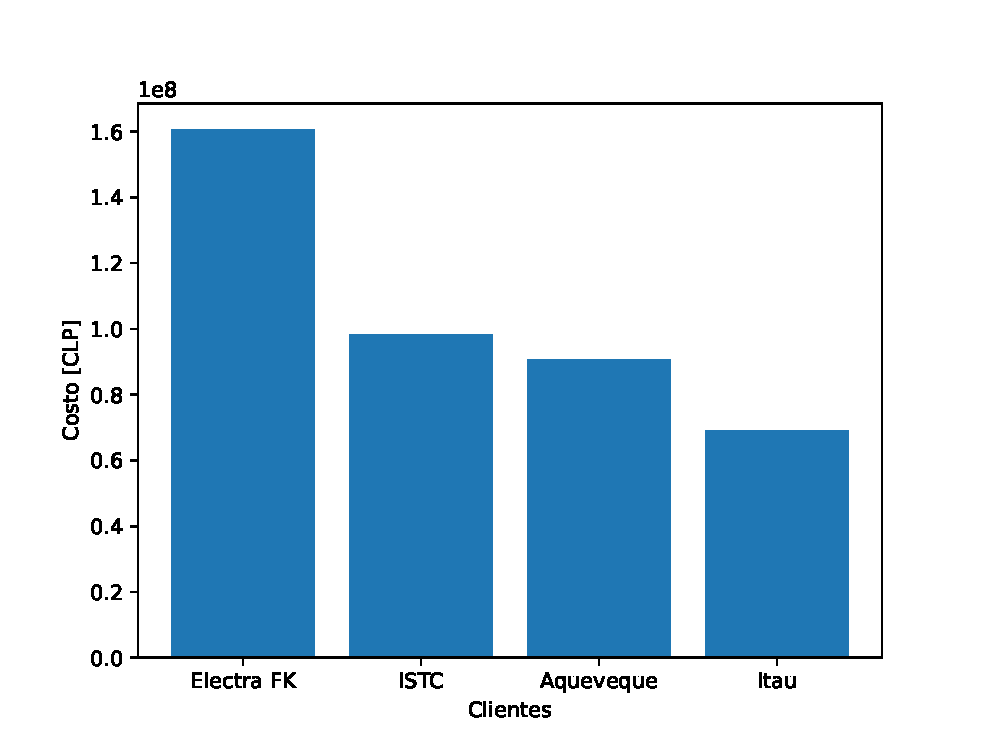
\includegraphics[width=0.8\textwidth]{EPS/cliente_monto_total.eps}
     \caption{Monto total de cotizaciones por cliente.}
     \label{graph:monto_max_cliente}
\end{figure}
\column{.35\textwidth}

\begin{block}{Monto cotizaciones histórico$^{**}$}
\begin{itemize}
    \item  Electra FK : \$160.582.057
    \item  ISTC : \$98.347.698
    \item  Aqueveque: \$90.549.449
    \item  Itau : \$69.219.557    
\end{itemize}
\end{block}
\begin{block}{}
    \tiny{** Los datos históricos se refieren al mes de análisis y período de referencia.}
\end{block}

\end{columns}
    
\end{frame}
%------------------------------------------------------------------
\usebackgroundtemplate{ 
\begin{figure}
        
\includegraphics[width=1.1\textwidth,height=1  \paperheight]{background/fondo_final2_50.jpg}
\end{figure}
}

\begin{frame}{}
\begin{center}
    
\includegraphics[width=0.4\textwidth]{background/ondyne_logo.png}\\
    \Large{\textbf{Diseñamos y protegemos tu energía.}}\\
    \small{Energía solar, sistemas UPS, baterías de litio, climatización precisa, control y monitoreo.}\\
\end{center}
\end{frame}

\end{document}